
\chapter{System Description}
\label{chapter:description}

\section{Overview}

The implemented data acquisition system was designed to collect medically relevant data and display it in real time through a web interface. This allows medical teams to permanently monitor patients and access patient's information remotely, including real time data and also the history of past values, allowing to detect patterns associated with certain diseases and monitor the progression or even check medication effectiveness.
Being completely mobile the system allows for a constant monitoring of hospitalized and non-hospitalized patients for periods that can go up to two months without the need for any maintenance, except for charging devices' battery obviously.
The system in prepared to deal with any numerical variables that can be collected with any sensor that has a \ac{bt} interface. This makes for a versatile completely in what sensors it can interact with and, thus what variables it can acquire, which make it suitable for almost all situations where pervasive long term monitoring can be useful.

Incoming data from sensors is collected into a smartphone that sends it, via web, to a central server that stores the data and serves the web interface. Physicians can specify which sensors should be active with each patient and which are the relevant variables to be acquired and displayed.

\begin{figure}[!h]
	\centering
	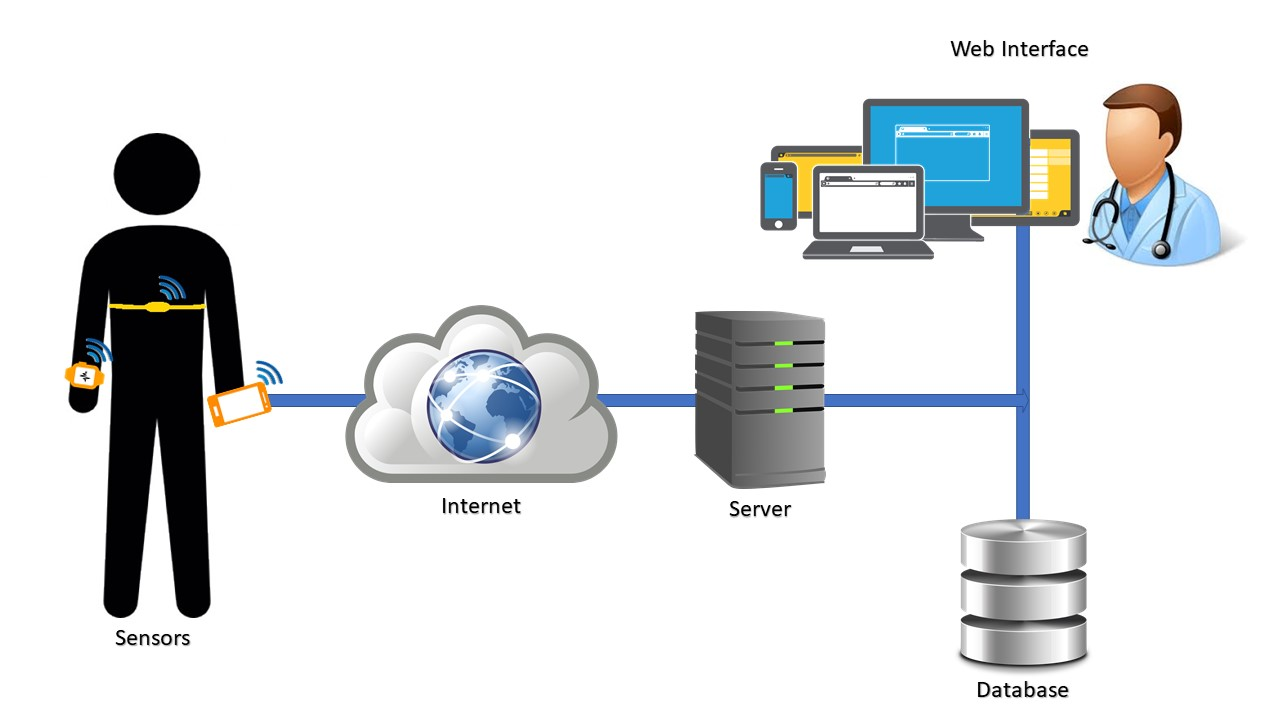
\includegraphics[width=\textwidth]{overview.jpg}
	\caption{System's architecture. Bluetooth connectivity between wearable devices. Smartphone connects to server through mobile web connection.}
	\label{fig:overview}
\end{figure}



The system works by having a physician configure all the acquisition parameters relevant for a certain patient and after this step no further intervention is needed, apart from equipping the patient and turning devices on. Parameters that can be configured are:
\begin{itemize}
	\item The type of devices currently available in the system (smartphone, smartwaches, etc...)
	\item What devices are to be given to the patient;
	\item What variables are to be collected from each device, and with what frequency they should be sent to the central server;
	\item The variables that are expected to be received by the server (that may not be the ones collected, some processing can occur) and how they should be visualized (color, range, etc...)
	\item Several alarms can be set defining what variable should be in what range for how long to trigger the alarm e.g. heart rate is below 50\ac{bpm} for more than 5 minutes;
\end{itemize}
This information is saved into the database. After the smartphone is turned on, information is retrieved from the server and acquisition starts. Until the end of the study data is continuously sent to the server where the physician can analyze it in real time (which is actually a 30s delay that is irrelevant for clinical practice.)

\begin{figure}[!h]
	\centering
	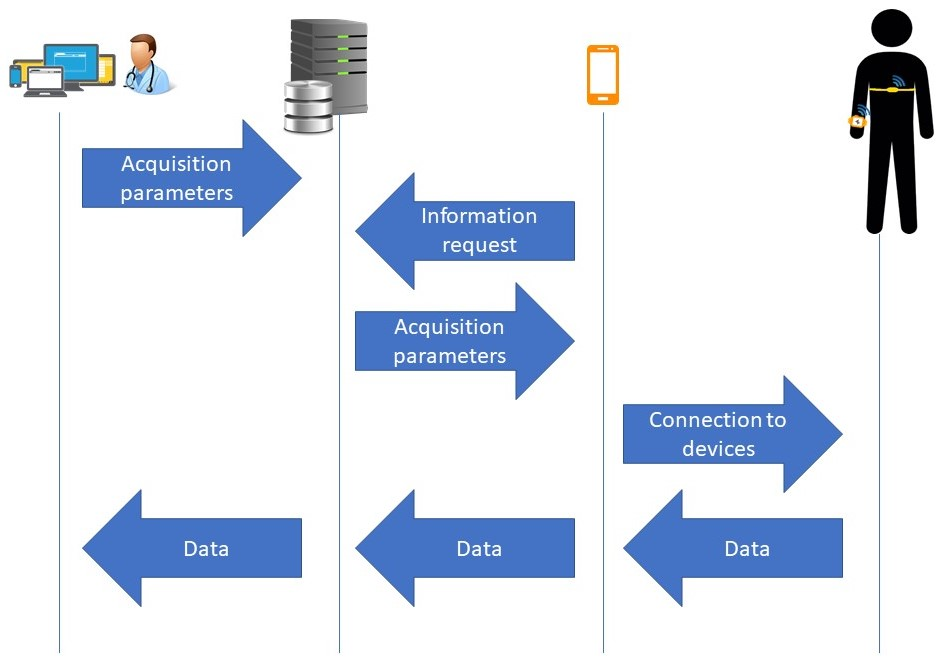
\includegraphics[width=\textwidth]{overview_info.jpg}
	\caption{System's data flow overview. Bluetooth connectivity between wearable devices. Smartphone connects to server through mobile web connection.}
	\label{fig:overview2}
\end{figure}

%Due to the multiplicity of devices used, several independent software components were developed to interact with each device and with the various sensors as illustrated in \cref{fig:platforms}.

\Cref{fig:overview} illustrates the general system architecture, where the local sensor network connects to a smartphone that relays information through web to a central server that manages the database and the web interface accessible to medical teams. \Cref{fig:overview2} depicts the timeline of communications between devices. Initially the user specifies the parameters in the interface that are stored in the database. When devices are turned on the smartphone pings the server which answers with the user configurations so it can start the communication with the configured sensors. After this the flow becomes mostly unidirectional with data coming from the sensors being relayed by the smartphone (eventually with some processing happening before) to the server then to saved into the database and displayed in the user interface when required.


%\FloatBarrier

\section{Devices}



\FloatBarrier
\subsection{Smartphone}

The smartphone is used to centralize data from the various sensors and as a local storage and processing unit. It receives all the raw data collected from the connected sensors, stores it into an \ac{sd} memory card, applies the necessary algorithms to extract information from the raw signals and finally sends this computed quantities to a central server so they can be visualized through a web interface.

All the sensors' data is transmitted through a Bluetooth interface and is stored as an array so it can be used to make the necessary calculations. Every 10s the data is saved into files stored in an \ac{sd} memory card. Data to be saved consists of time-series composed by consecutive data samples from the sensors. This samples are acquired at different rates from each sensor and a timestamp is associated to each sample in order to facilitate the time location of each one and make easier to align the signals from different sensors. The app is prepared to deal with any number of sensors per connected device and it stores data in a separate file for every remote device, containing data from all the device's sensors.


%\begin{figure}[!h]
%	\centering
%	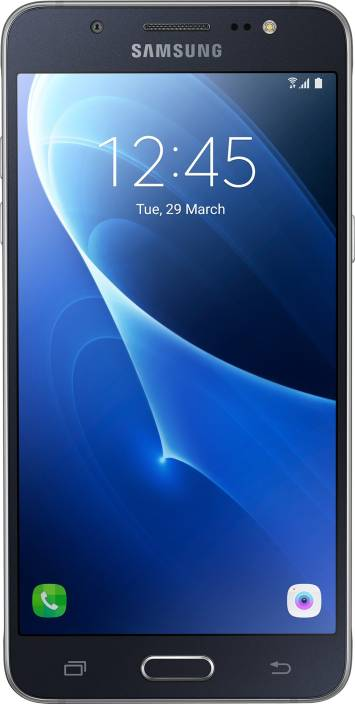
\includegraphics[width=0.2\textwidth]{samsung-j5.jpeg}
%	\caption{Smartphone Samsung J5}
%	\label{fig:phone}
%\end{figure}

\subsubsection{Android App}

The android app was implemented using Android Studio 3.0.1. All functions were designed to be as computationally efficient as possible to minimize time delay and maximize battery life. The app was designed as a replacement of the android home screen, so when the smartphone is turned on, the app will automatically initiate and show on screen, ensuring the patient does not forget to initiate it. Another focal point of the implemented app is the thread-oriented logic that eases future development and new sensors integration. This means that support and communication for each sensor runs in an independent thread, easing the process of introducing support for new remote sensors.

At startup, in the main thread, the app checks for Internet and Bluetooth connectivity, requesting its activation if necessary. A background service is initiated and it will be responsible for all the non-display actions. This was necessary not to crash the display as background tasks can be time consuming and will need to run even if the display is deactivated or if the screen is locked.
The background service then starts its task by establishing a socket \cite{tcpip} to the server @learnib.lx.it.pt and sending the smartphone's \ac{uuid} which is the Wi-Fi mac address. Initially the Bluettoth adapter address was to be used as \ac{uuid} for the smartphone, but recent versions of Android \ac{os} do not allow to programmatically get it so, alternatively, Wi-Fi mac address was used. 

\FloatBarrier

Code used to determine smartphone's mac address:

\bigskip
\begin{lstlisting}[language=Java]
import android.annotation.TargetApi;
import java.net.NetworkInterface;
import android.bluetooth.BluetoothAdapter;
import java.util.List;


@TargetApi(9)
public static String getMacAddr() {
	BluetoothAdapter bluetoothAdapter = BluetoothAdapter.getDefaultAdapter();
	if(bluetoothAdapter == null){
		return null;
	}	
	String addr = bluetoothAdapter.getAddress();	
	try {
		if (addr.equals("02:00:00:00:00:00")) {		
			List<NetworkInterface> all = Collections.list(NetworkInterface.getNetworkInterfaces());
			for (NetworkInterface nif : all) {
				if (!nif.getName().equalsIgnoreCase("wlan0")) continue;			
				byte[] macBytes = nif.getHardwareAddress();
				if (macBytes == null) {
					return "";
				}
				StringBuilder res1 = new StringBuilder();
				for (byte b : macBytes) {
					res1.append(String.format("%02x", b) + ":");
				}				
				if (res1.length() > 0) {
					res1.deleteCharAt(res1.length() - 1);
				}
				Log.d(TAG, "MAC ADRSS: " + res1.toString());
				return res1.toString();
			}
		}
	} catch (Exception ex) { }
	return addr;
}
\end{lstlisting}
\bigskip

Connection to the server is made using java's native socket implementation:

\bigskip
\begin{lstlisting}[language=Java]
import java.net.Socket;

private Socket socket;
private OutputStream out;
private InputStream in;
private final String host = "learnbig.lx.it.pt";
private final int port = ********;

public void connect() {
	try {
		socket = null;
		out = null;
		in = null;
		socket = new Socket();		
		socket.connect(new InetSocketAddress(this.host,this.port), 10000);
		out = socket.getOutputStream();
		in = socket.getInputStream();
	}
	catch (Exception e) {}
	catch (Throwable t) {}
}
\end{lstlisting}
\bigskip

After the socket is connected, the \ac{uuid} is sent to the server that replies with a message containing the Bluetooth mac addresses of all the remote devices and sensors that the smartphone should connect to. It also sends the information about the frequency at which data should be sent to the server and, if necessary, other device-specific parameters. In case of connection failure the background service sends this information using a previously registered ResultReceiver causing the \ac{ui} activity to change the background color and send a notification with sound to the user while simultaneously retrying to connect.

As this information is received and parsed, the necessary devices are initialized. A different class is implemented to interact with each type of device, as different communication protocols are required. Each of this classes extends the native Thread class in order to have complete independence between devices. This aspect enhances the versatility of the system, easing the implementation of support for new sensors. This is also needed to avoid clogging the processor and the Bluetooth reading buffers, as events occur asynchronously between devices and timing is relevant to ensure no data is lost.

\begin{figure}[!h]
	\centering
	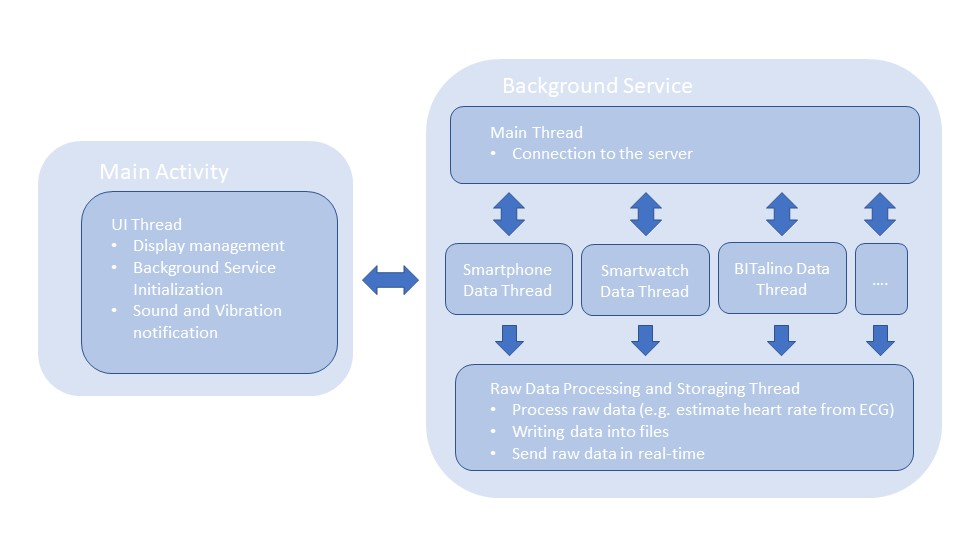
\includegraphics[width=\textwidth]{app_android.jpg}
	\caption{Android App threads call-stack}
	\label{fig:app_thread}
\end{figure}

Device's classes all work in similar ways. They establish a Bluetooth connection and handle the incoming data. As sensor values reach the smartphone, they are stored into buffers holding 10s of data. When buffers are full, the 10s window of data is compressed and saved into a file and the data is processed in order to extract medically relevant indicators like the \ac{hr} for example which are then displayed in the \ac{ui} thread. Saving data into the files is accomplished using BufferedWriter and StringBuilder classes for optimized performance \cite{android}. BufferedWriter class uses a non blocking write that allows the device thread to continue his strenuous work without much delay. StringBuilder class is used in order to compose the strings that ought to be saved without the need to allocate new memory blocks with each append as it would be necessary if dealing with Strings. Data is saved into an \ac{sd} card or to the smartphone memory if the early is not present. All file writing processes are synchronized to protect against a case where two threads are reading or writing to the same file at the same time.

\Cref{fig:app_thread} illustrates the general architecture of the implemented app, showing the two services with their threads. Background service, as refered before, has a main thread that establishes connection to the server, than a separate thread to interact with each device and finally a thread to save and process data. 


Data is saved to files in a specific format detailed in \cref{chapter:compresion} and the code utilized to save it most efficiently is as follows:

\bigskip
\begin{lstlisting}[language=Java]
import java.io.BufferedWriter;
import java.io.File;
import java.io.FileInputStream;
import java.io.FileNotFoundException;
import java.io.FileReader;
import java.io.FileWriter;
import java.io.IOException;
import java.nio.*;

private BufferedWriter bw = null;
private File file;

public open_file(Context ctx, String device, String person_ID) {

	context = ctx;
	this.person_ID = person_ID;
	File[] paths = context.getExternalFilesDirs(null);
	File path;
	int n = 0;
	
	if (paths.length == 2) {
		path = paths[1];
	} else {
		path = paths[0];
	}
	
	file = new File(path, device + "_" + person_ID + ".txt");
	
	try {
		bw = new BufferedWriter(new FileWriter(file, true));
	} catch (IOException e) {
		e.printStackTrace();
		Log.d(TAG, "Erro erro ao abrir o writer");
		try {
			file.createNewFile();
			bw = new BufferedWriter(new FileWriter(file, true));
		} catch (Exception ex) {
			Log.d(TAG, "Erro erro ao abrir o writer depois de criar o ficheiro");
			e.printStackTrace();
		}
	
	}
	
	Log.d(TAG, "Iniciou com sucesso");
}

public void insert_data_list(int[] RAWmeasurementsArray, Long[]  RAWtimestampsArray) {

	StringBuilder str = new StringBuilder();
	int buf = 0;
	Long buf_time = 0L;
	String separator = ";";
	
	str.append("#");
	str.append(separator);
	
	for (int i = 0; i < RAWmeasurementsArray.length; i++) {
		str.append(String.valueOf((Long) RAWtimestampsArray[i] - buf_time));
		buf_time = (Long) RAWtimestampsArray[i];	
		str.append(separator);
		str.append(String.valueOf(RAWmeasurementsArray[i] - buf));
		buf = RAWmeasurementsArray[i];
	}
	str.append("\n");
	
	synchronized (bw) {
	
		try {
			bw.write(str.toString());
		} catch (IOException e) {
			e.printStackTrace();
			Log.d(TAG, "Erro ao escrever ficheiro");
			try {
				bw[this.index] = new BufferedWriter(new FileWriter(files[this.index], true));
			} catch (IOException e1) {
				e1.printStackTrace();
				Log.d(TAG, "Erro ao abrir ficheiro");
			}
		}
	}
	
	str = new StringBuilder();
	
	try {
		bw.flush();
	} catch (IOException e) {
		e.printStackTrace();
		try {
			bw = new BufferedWriter(new FileWriter(file, true));
		} catch (IOException e1) {
			e1.printStackTrace();
		}
	}
}


\end{lstlisting}
\bigskip


Optionally, using the web interface, user can request raw data in real time from a specific or all devices to be sent. This process is accomplished by a separate thread that receives each 10s block of data that is written to files, further compresses and sends it through a socket to the server where data is stored.
Further compression is needed as bandwidth and internet plafond are more restrictive than memory space. Data compression and sending occurs in a separate thread to ensure there is no delay in data acquisition.

At the same time data is saved into files by each device's thread, the result of processing that 10s window of data is sent to the \ac{ui} thread to be displayed on screen. These threads also request battery status from the devices. This information is sent to the \ac{ui} thread where a symbol indicates battery status of each device.

To summarize, raw data coming from the sensors is stored into files and optionally sent to the server. That same data is then processed to extract more relevant and 
informative measures, that are again sent to the server and shown in the smartphone screen alongside with battery status and Bluetooth connection status. \Cref{fig:app} shows the main screens of the app with the main stages of initialization (\cref{fig:app1,fig:app2,fig:app3}) and when connection to the server cannot be made (\cref{fig:app4}).


\begin{figure}[!t]
	\centering
	\makebox[\linewidth][c]{%
		\begin{subfigure}[t]{0.5\textwidth}
			\centering
			\captionsetup{width=.75\linewidth}
			\fbox{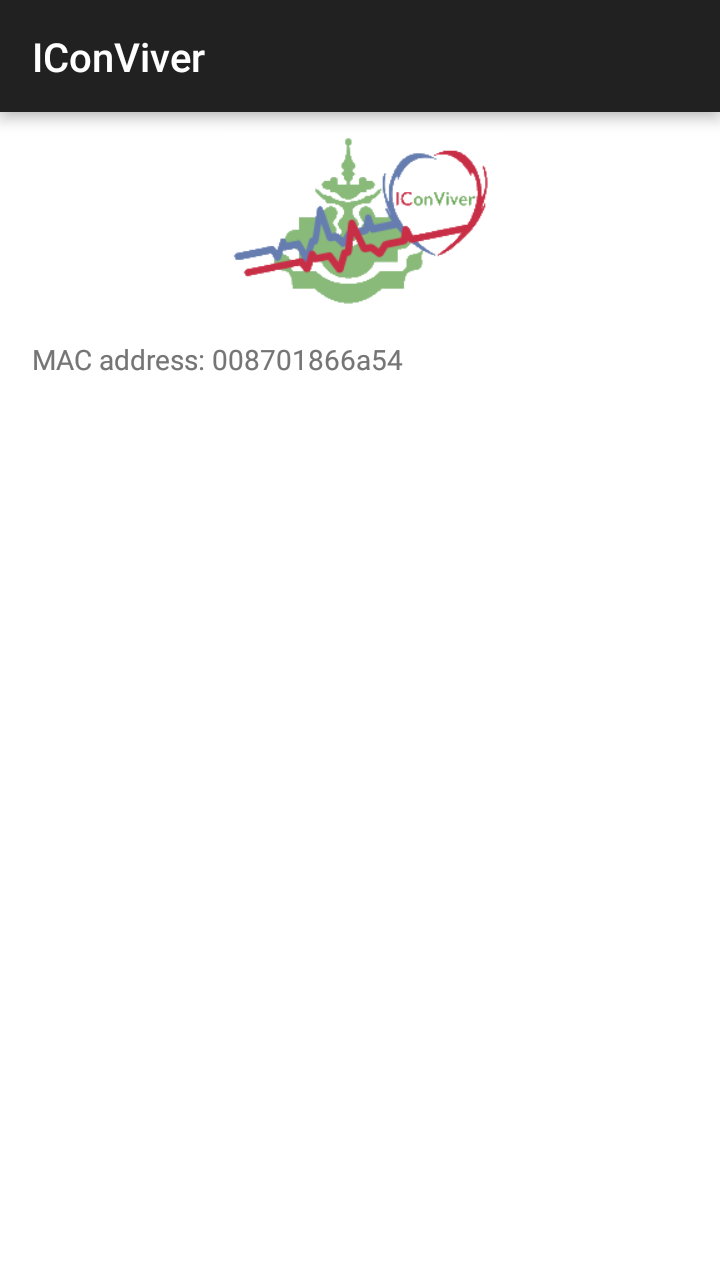
\includegraphics[width=0.6\textwidth]{screen_on.png}}
			\caption{Display at startup showing device's \ac{uuid}}
			\label{fig:app1}
		\end{subfigure}%
		\begin{subfigure}[t]{0.5\textwidth}
			\centering
			\captionsetup{width=.75\linewidth}
			\fbox{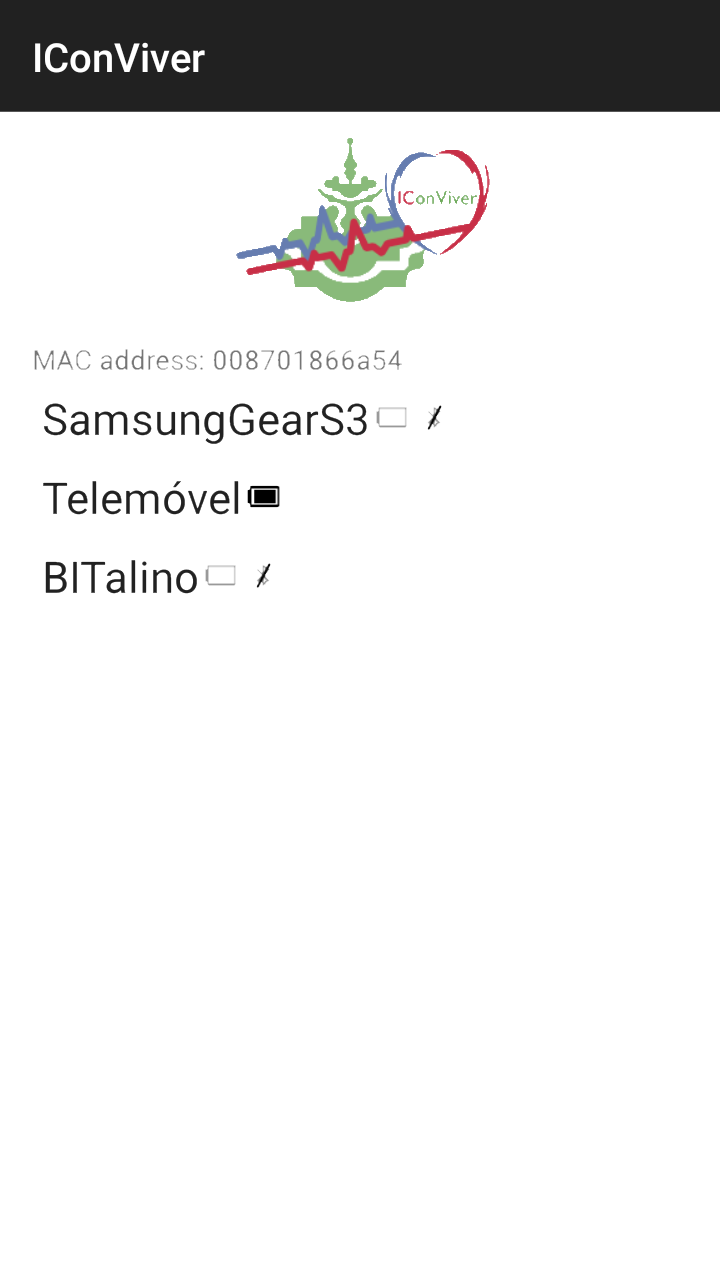
\includegraphics[width=0.6\textwidth]{screen_on1.png}}
			\caption{Display after information from the server is received. Bluetooth symbols indicate there is still no connection with peripheral devices.}
			\label{fig:app2}
		\end{subfigure}%
	}\\
	\makebox[\linewidth][c]{%
		\begin{subfigure}[t]{0.5\textwidth}
			\centering
			\captionsetup{width=.75\linewidth}
			\fbox{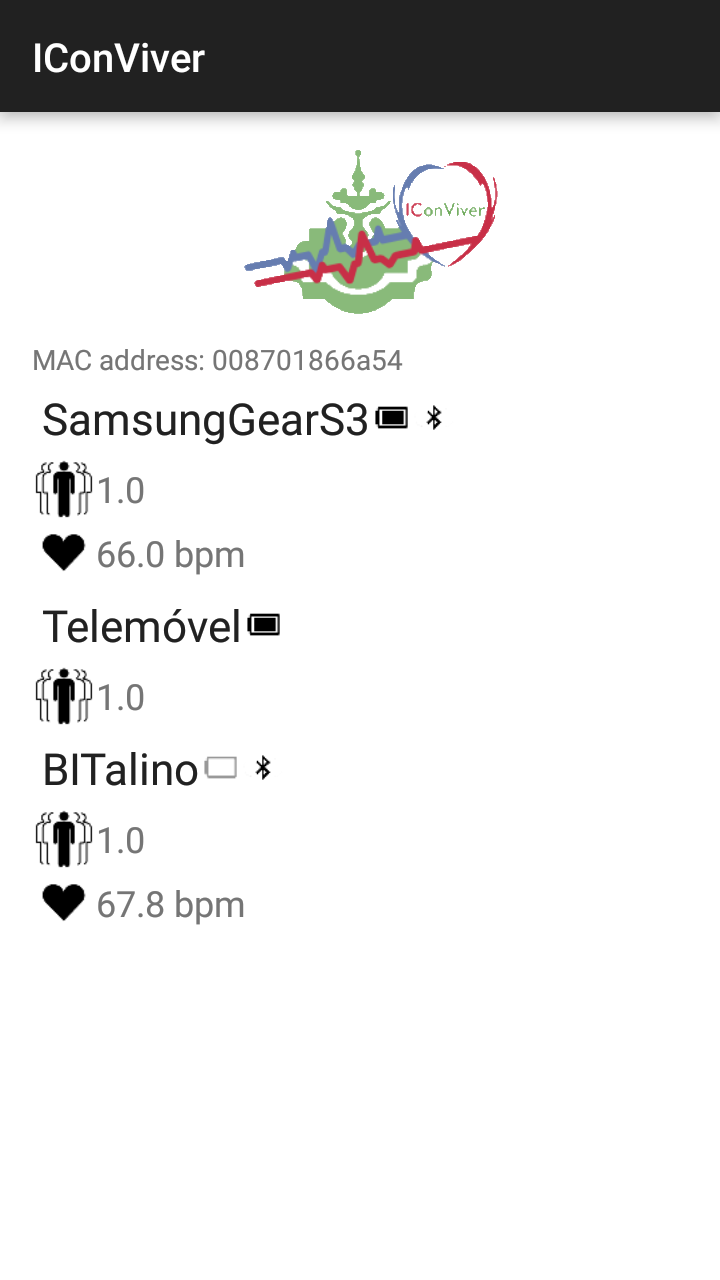
\includegraphics[width=0.6\textwidth]{screen_on2.png}}
			\caption{Display after connection has been established and data from devices is received. Below each device's name there is the value resulting from processing the last 10s of data collected.}
			\label{fig:app3}
		\end{subfigure}%
		\begin{subfigure}[t]{0.5\textwidth}
			\centering
			\captionsetup{width=.75\linewidth}
			\fbox{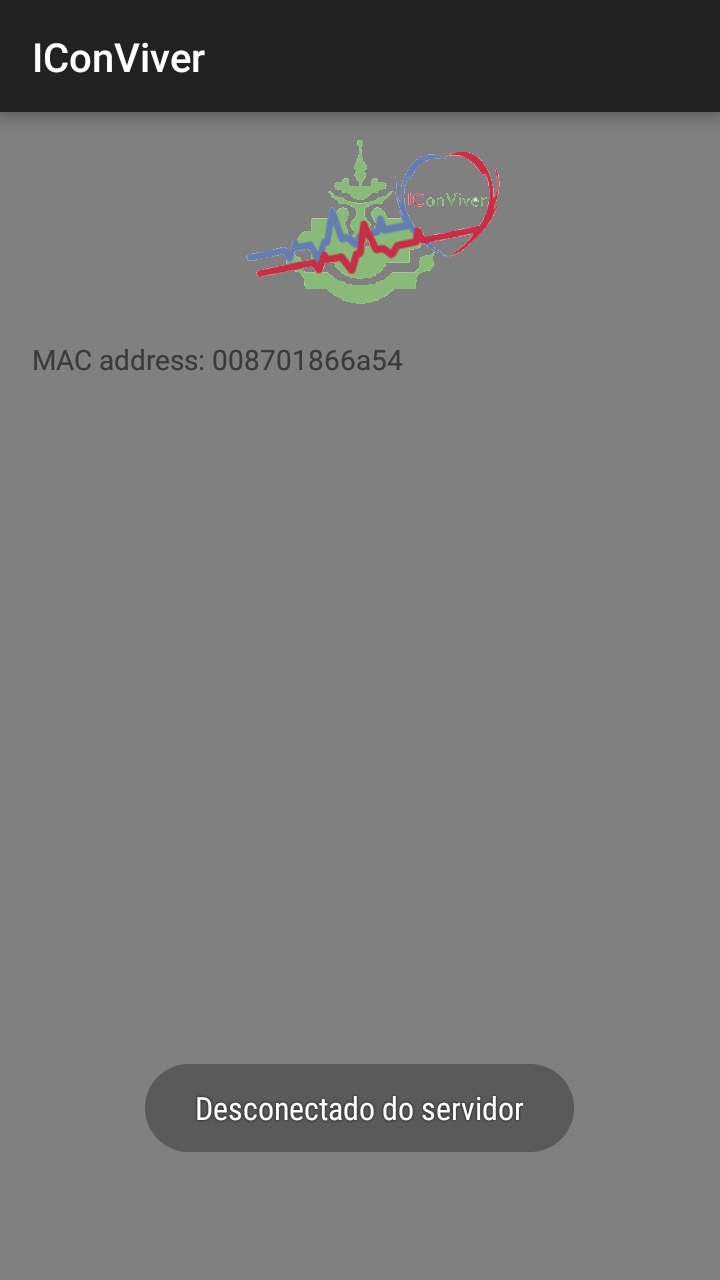
\includegraphics[width=0.6\textwidth]{screen_off.png}}
			\caption{Screen when it was not possible to establish server connection. A sound notification also occurs in this event.}
			\label{fig:app4}
		\end{subfigure}%
	}\\
	\caption{Android App screen in different situations.}
	\label{fig:app}
\end{figure}

In case any Bluetooth connection to any remote device is lost, the corresponding device's thread will try to reconnect it indefinitely and will trigger a notification with sound and an icon will appear in the app screen informing the user connection is lost. This is useful in case the user is not wearing one of the devices and forgets it. Also a warning message will be sent to the server and a mark will appear in data visualization, informing the medical teams of the momen the device was disconected. All threads and procedures will proceed normally when the lost connection is reestablished. In case the server connection is lost, background service's main thread will also try to reconnect indefinitely, leaving all other threads running with no interference. When reconnected, all other threads are stopped and the call-stack is restarted as if the app was just initialized. This occurs in this way to ensure that data acquisition continues even if the patient enters an area with no mobile data communication and, ant the same time, when the communication is reestablished, acquisition restarts to preclude any change in acquisition parameters. When the app cannot communicae with the server, or server is lost, a notification is emmited and the background color of the home screen changes.



\FloatBarrier

\subsection{Server and Web Interface}

\bigskip
\textcolor{red}{\Large \textbf{Pôr as figuras num anexo em vez de aqui no meio do texto?}}
\bigskip

\begin{figure}[h!]
	\centering
	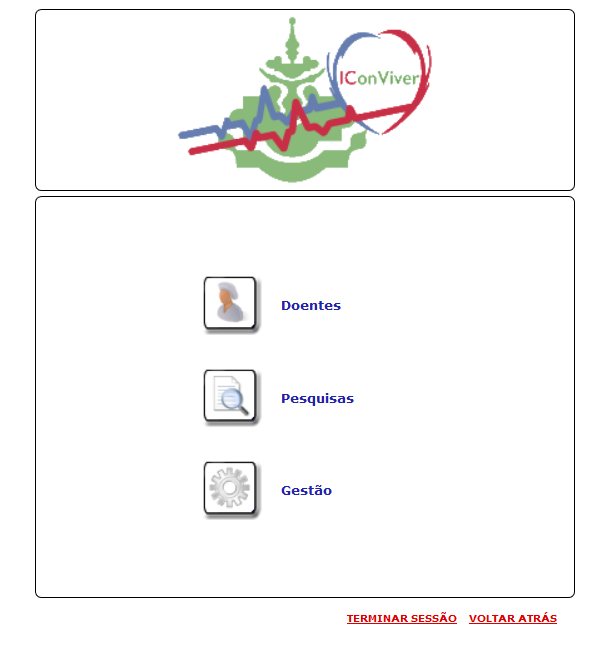
\includegraphics[width=0.45\textwidth]{login2.png}
	\captionsetup{width=0.4\textwidth}
	\caption{Initial panel after login into the system's web interface. Here one can see patient information; search for specific data of a particular patient; configure all device and acquisition parameters.}
	\label{figure:UI1}
	
\end{figure}%

\begin{figure}[h!]
	\centering
	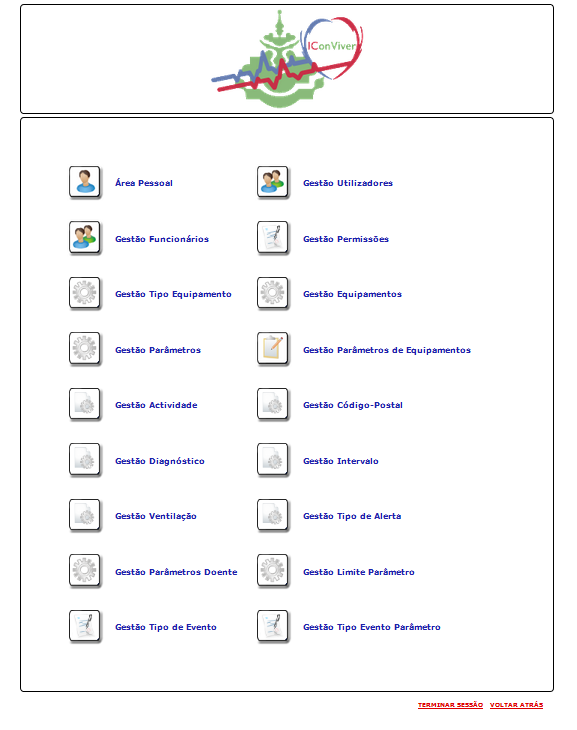
\includegraphics[width=0.85\textwidth]{gestao.png}
	\captionsetup{width=0.8\textwidth}
	\caption{Management screen, where all the systems and device's parameters can be defined.}
	\label{figure:UI_gestao}
	
\end{figure}%

\begin{figure}[h!]
	\centering
	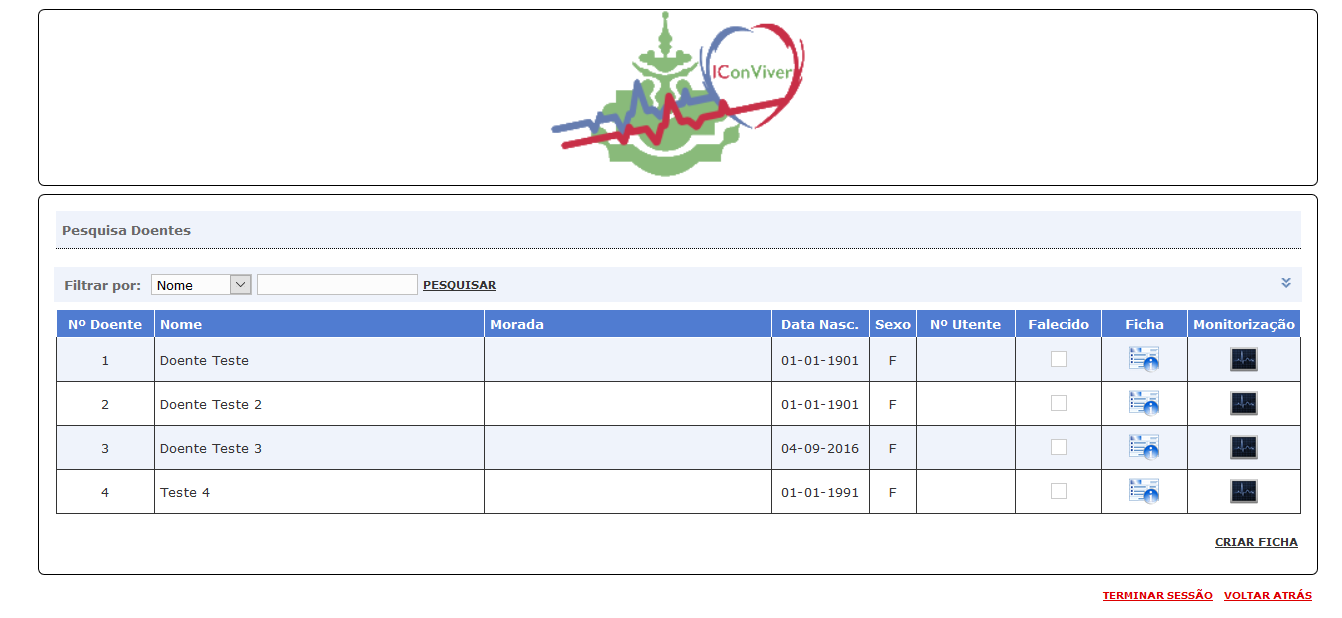
\includegraphics[width=0.85\textwidth]{doentes2.png}
	\captionsetup{width=0.8\textwidth}
	\caption{Screen showing the patients enrolled in the system. From here one can access all the information and collected data from each patient.}
	\label{figure:UI2}
\end{figure}%


\begin{figure}[h!]
	\centering
	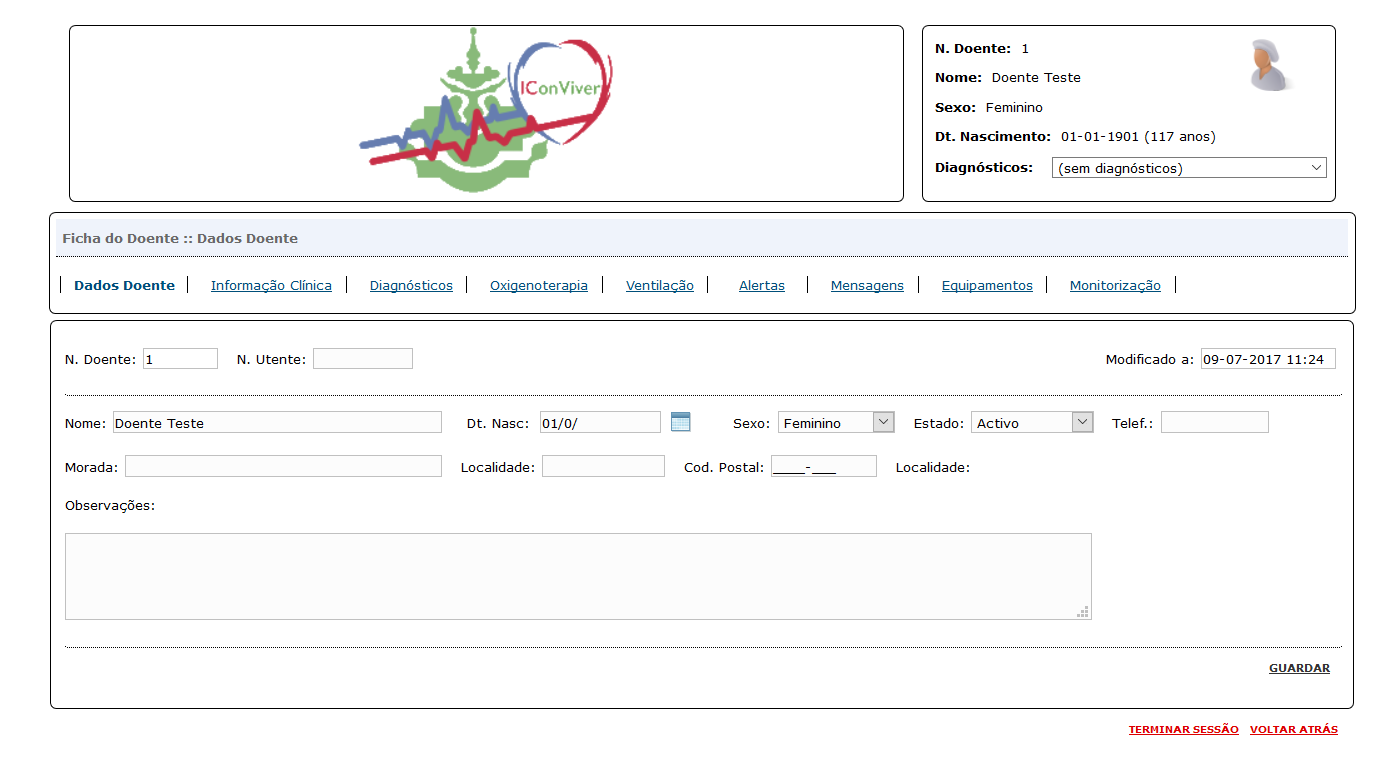
\includegraphics[width=0.85\textwidth]{paciente.png}
	\captionsetup{width=0.8\textwidth}
	\caption{Data visualization screen where one can choose the variables to see and their time frame.}
	\label{figure:UI4}
\end{figure}%

\begin{figure}[h!]
	\centering
	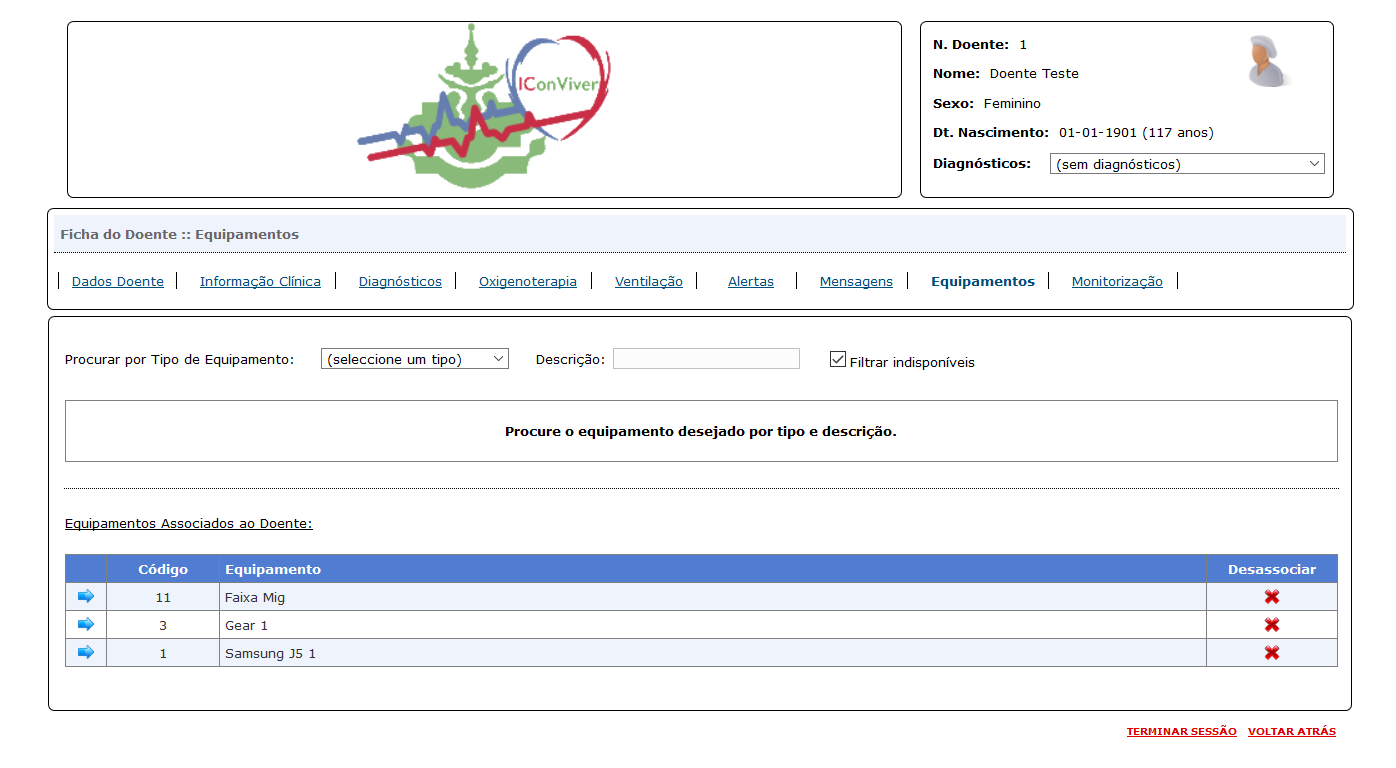
\includegraphics[width=0.85\textwidth]{dispositivos.png}
	\captionsetup{width=0.8\textwidth}
	\caption{Data visualization screen where one can choose the variables to see and their time frame.}
	\label{figure:UI5}
\end{figure}%

\begin{figure}[h!]
	\centering
	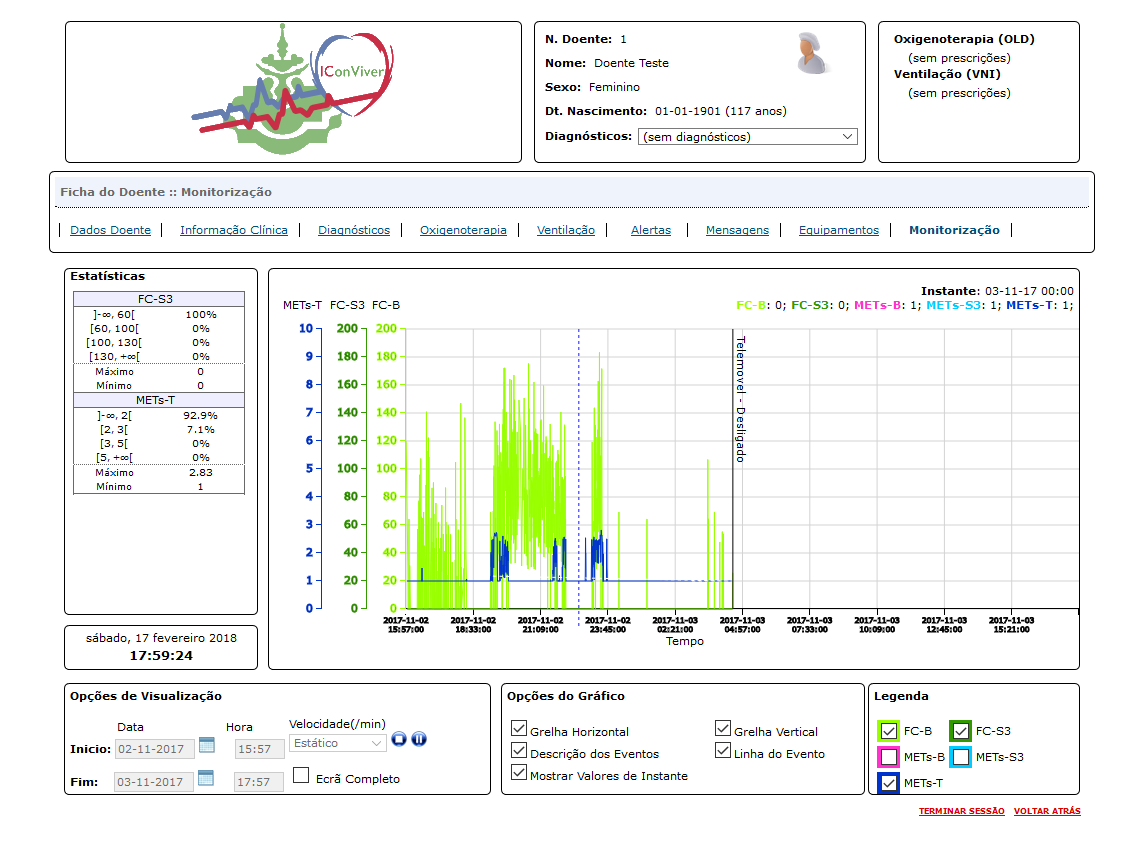
\includegraphics[width=0.75\textwidth]{data3.png}
	\caption{Data visualization screen where one can choose the variables to see and their time frame.}
	\label{figure:UI3}
\end{figure}%

Software for the server was adapted from software already implemented  for a different project \cite{telemold} by \ac{insticc}. All parameters and information to be passed to the remote device can be configured using the web interface and any numerical data coming from it can be shown in an interactive panel as well as warnings and events.

All aspects of the \ac{ui} were designed to provide a simple and versatile interface that can be used to interact with very different types of variables coming from a multitude of sensors. The main goal was to have a single interface that could be used in various contexts inside and out of hospital applications, and capable of being easily used with many variables and sensors.

The server itself is a computer with windows operative system and an internet connection that acts as a central control unit for the whole system. It is responsible for serving the user web interface, relaying information between the user and the devices and finally store all the information into a database. The interface is based in the .NET framewok with a Windows SQL Database.

System works with three major components:

\begin{itemize}
	\item \textbf{Web interface -} This is an ASP.NET website served using Windows Internet Information Services where user can configure all patient, device and acquisition parameters that are then stored into the database
	\item \textbf{Socket -} This component is in fact the two different subcomponents that ensure the communication between remote devices and the database.
	\begin{itemize}
		\item A .NET script is constantly waiting for socket connections and sends acquisition parameters to remote devices. It also receives and stores data sent from the devices containing patient processed data like \ac{hr} and \ac{mets} values.
		\item A Python script also constantly waiting for socket connections in a different port. This script is responsible for receiving and storing realtime raw data that may be sent by remote device (only active if raw data is requested).
	\end{itemize}
	\item \textbf{Database -} This component is responsible for receiving and storing all data that comes from all other components.
\end{itemize}

Two different socket processes were implemented to prevent clogging which could lead to data being lost. Also different languages were used for implementation convenience.

%\bigskip
%\textcolor{red}{\Large \textbf{Incompleto, imagens dos paineis e lista das costumizaçoes que podem ser feitas}}
%\bigskip

%\begin{figure}[h!]
%	\centering
%	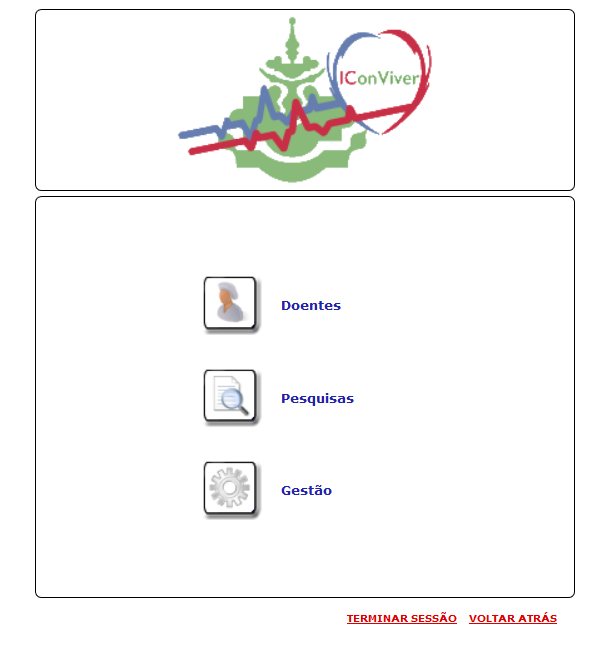
\includegraphics[width=0.45\textwidth]{login2.png}
%	\captionsetup{width=0.4\textwidth}
%	\caption{Initial panel after login into the system's web interface. Here one can see patient information; search for specific data of a particular patient; configure all device and acquisition parameters.}
%	\label{figure:UI1}
%	
%\end{figure}%
%
%\begin{figure}[h!]
%	\centering
%	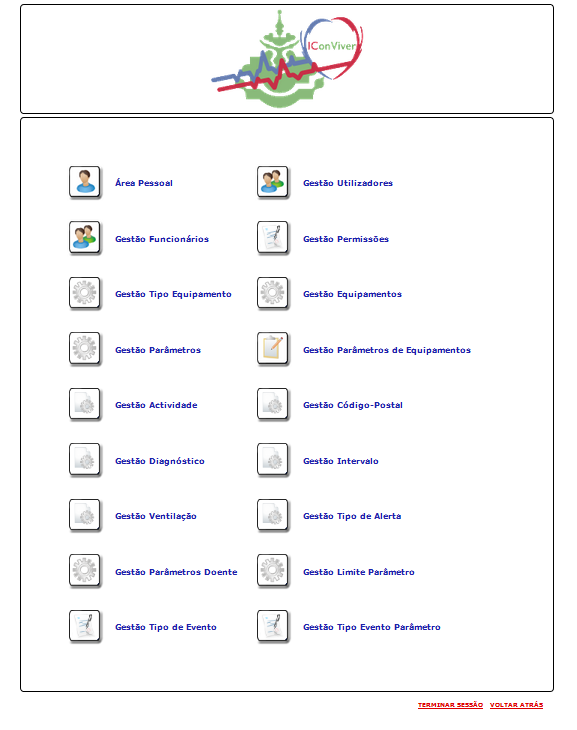
\includegraphics[width=0.85\textwidth]{gestao.png}
%	\captionsetup{width=0.8\textwidth}
%	\caption{Management screen, where all the systems and device's parameters can be defined.}
%	\label{figure:UI_gestao}
%	
%\end{figure}%
%
%\begin{figure}[h!]
%	\centering
%	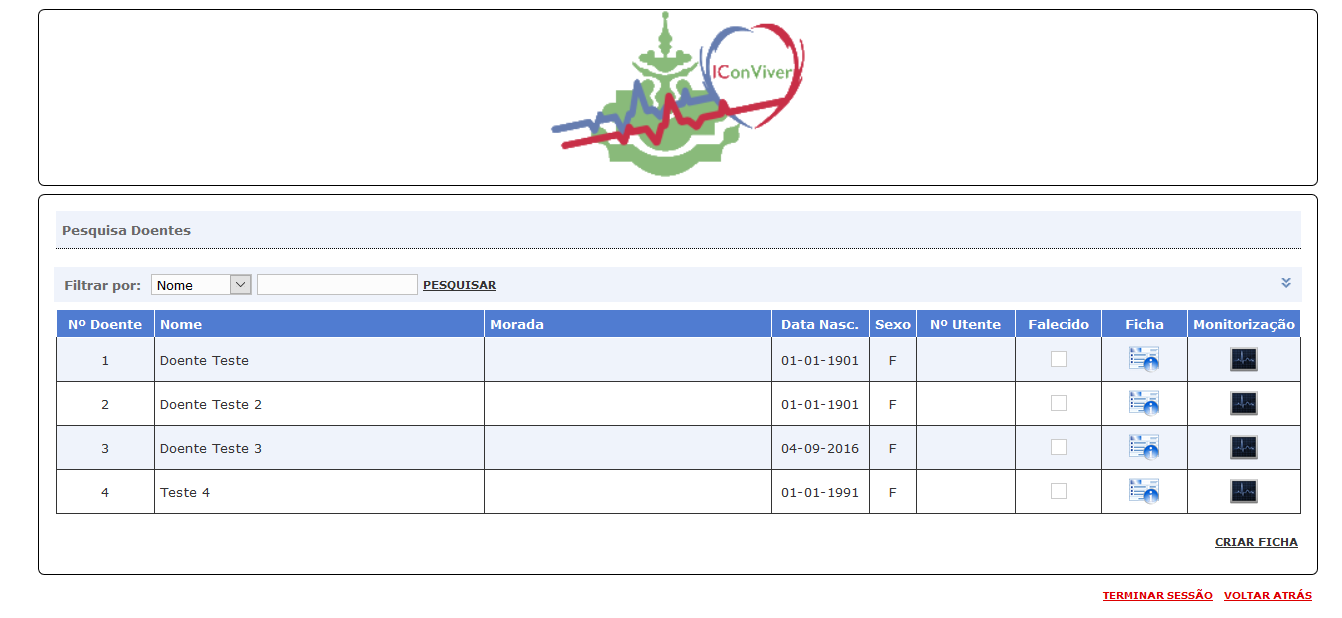
\includegraphics[width=0.85\textwidth]{doentes2.png}
%	\captionsetup{width=0.8\textwidth}
%	\caption{Screen showing the patients enrolled in the system. From here one can access all the information and collected data from each patient.}
%	\label{figure:UI2}
%\end{figure}%
%
%
%\begin{figure}[h!]
%	\centering
%	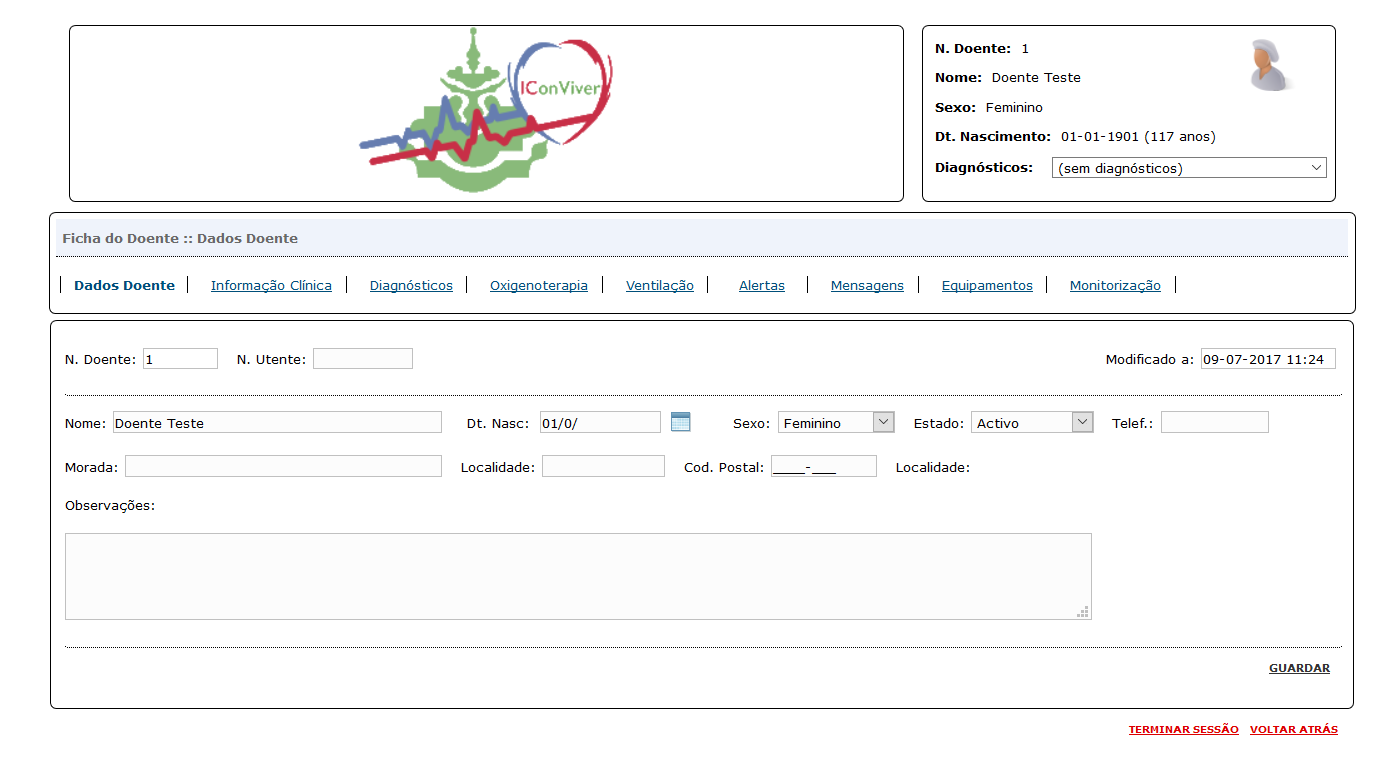
\includegraphics[width=0.85\textwidth]{paciente.png}
%	\captionsetup{width=0.8\textwidth}
%	\caption{Data visualization screen where one can choose the variables to see and their time frame.}
%	\label{figure:UI4}
%\end{figure}%
%
%\begin{figure}[h!]
%	\centering
%	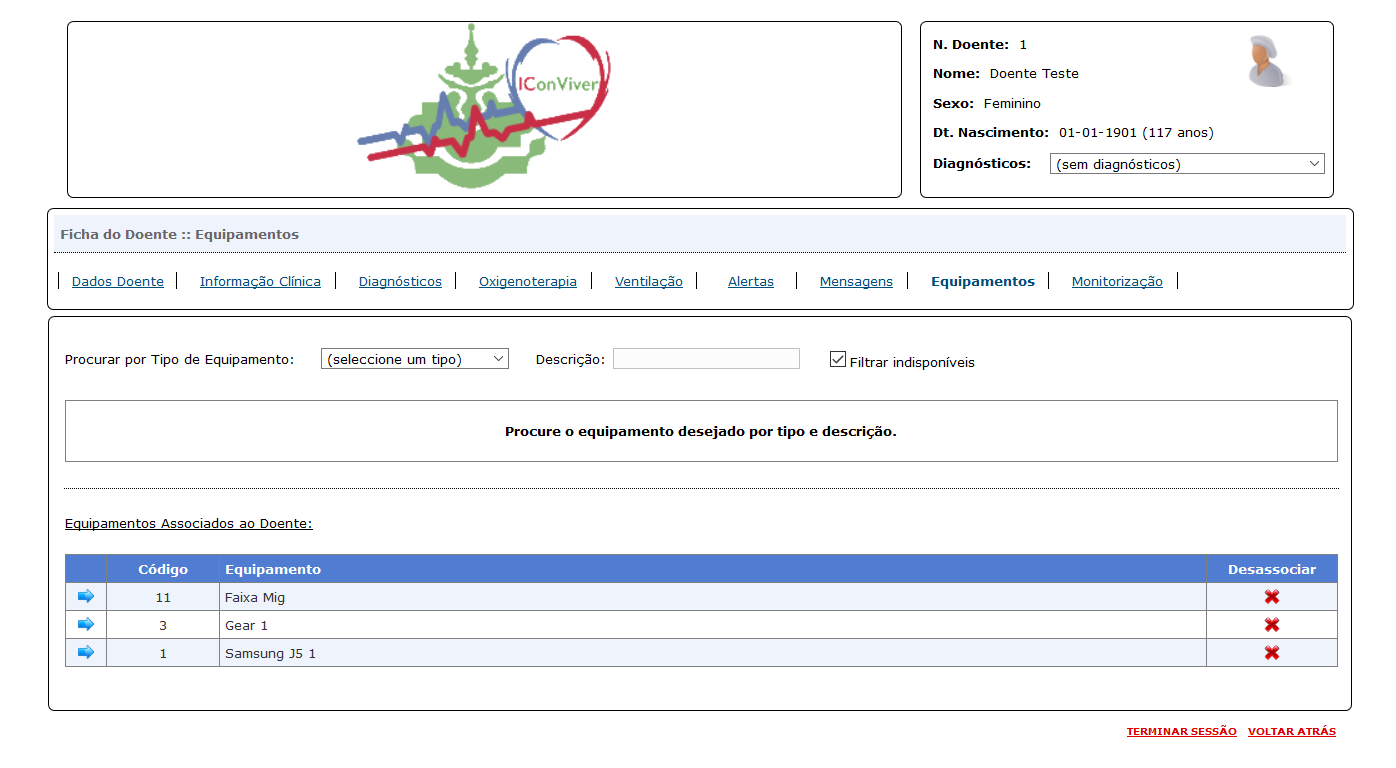
\includegraphics[width=0.85\textwidth]{dispositivos.png}
%	\captionsetup{width=0.8\textwidth}
%	\caption{Data visualization screen where one can choose the variables to see and their time frame.}
%	\label{figure:UI5}
%\end{figure}%
%\begin{figure}[h!]
%	\centering
%	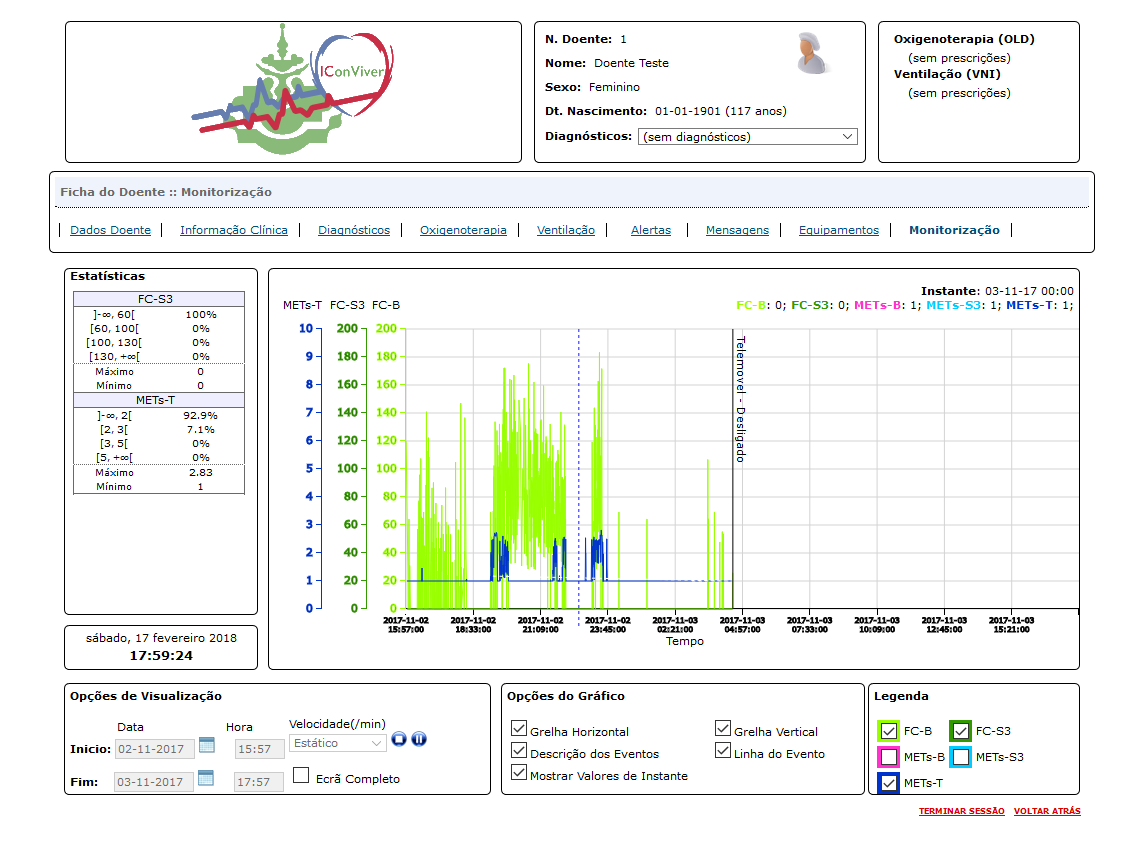
\includegraphics[width=0.75\textwidth]{data3.png}
%	\caption{Data visualization screen where one can choose the variables to see and their time frame.}
%	\label{figure:UI3}
%\end{figure}%

\Cref{figure:UI1,figure:UI_gestao, figure:UI2,figure:UI3,figure:UI4,figure:UI5} show some examples of the implemented web user interface, from where medical teams can control and configure all stages of the patient monitoring. From this interface medical teams can configure and access all information in the system ensuring the system is versatile to deal with many use cases.

\FloatBarrier
\subsubsection{Initial Server Configuration}



In order to setup the system to start acquisition, some parameters need to be configured in the management (Gestão) screen showed in \cref{figure:UI_gestao} that are accessed from screen in \cref{figure:UI1} after successful login.

Parameters to be configured on system setup:

\begin{enumerate}
	\item Devices connected to the system are categorized into types like smartphones or chest bands or others. The names of these types of devices are completely configurable, but to prevent mistakes only one device of each type can be assigned to a patient simultaneously. Each type of devices is identified by a name and single character code e.g. an S for smartphones.
	
	\item For each type of device it is required to define which parameters they need, these parameters must include a key parameter that includes the \ac{uuid} of the device labeled with the identifier "I". Other parameters can be configured but they vary based on the implemented features and support from the Android app, however they tend to be related with what sensors are active in each remote sensors and with what frequency they acquire and transmit data. These parameters are sent to the smartphone when it is turned on and are interpreted or relayed to the remote devices depending on the implemented interactions.
	
	\item It is also required to define what variables are to be displayed in the data visualization screen from \cref{figure:UI3}. To do this user must define the name of the variable, its range and the color of the corresponding line in the plot panel. Furthermore user can define intervals of values to see later the percentage of data that lies inside those intervals. This statistics can be seen in left panel of \cref{figure:UI3}.
	
	\item Optionally medical teams can configure rules that trigger an notification e.g \ac{hr} is below 50\ac{bpm} for more than 2minutes. To configure this rules, one should select a variable, a reference value, a relation between them (\textless, \textgreater or =) and a duration.
\end{enumerate}

\subsubsection{Acquisition Start}

In order to start data acquisition it is necessary to add patient information in screen showed in \cref{figure:UI4} and add the devices that should be active with that patient in screen of \cref{figure:UI5}. After this step, the smartphone and all other devices can be turned on and acquisition starts with data being displayed in panel of \cref{figure:UI3}. As data is received from the remote devices, it is displayed and user can chose to see data from a specific time-interval or to see data as it arrives in real time. From the web interface it is also possible to send text messages to the smartphone given to the patient.

All this configuration steps are necessary to ensure compatibility with any sensor medical teams consider adequate, making the system able to deal with any peculiarities each sensor may have.

Steps necessary for rotine aquisition start are presented in \cref{apendix:userguide}.

\section{Communication Protrocol}

\Cref{apendix:system} Details this topic.

When the smartphone is turned on, the application starts its execution and sends an initial message to the server containing a timestamp and its own \ac{uuid}. The server then responds with n identic messages, where n is the number of remote/wearable sensors. These messages contain the code number of the patient, a timestamp, the UUID of the remote sensor, the type of the remote sensor (smartwatch, smartphone, etc...) and pairs of (name, value) for all the custom parameters that user defined in the configuration.
The first and last character of these handshake messages is the special mark "\textbackslash".

After this initial handshake, the smartphone periodically sends data to the server in a similar fashion, the message is composed of a timestamp, the patient code number and pairs of (name, value) for each of the variables that are being sent. For this messages, the first and last character is \#.

Other messages are exchanged including alerts and events, each type having a similar structure, timestamp, patient code, and pairs of values and identifications containing the UUID of the relevant device and the respective error or event code. Each type of message has a special character that is repeated in the begining and end of the message.

Regarding the communication between the remote sensors and the smartphone, this is a very variable protocol as it depends on the peculiarities of each sensor utilized, and for this reason no standard protocol is defined.

%The first message sent by the smartphone:
%
%%\begin{verbatim}
%%  \ 1417162942424 0019B9FBE258 \
%%  1      2             3       4
%%\end{verbatim}
%
%\begin{table}[h!]
%%	\small
%	\begin{tabular}{>{\color{pgrey}}c >{\color{pgrey}}c >{\color{pgrey}}c >{\color{pgrey}}c}
%		\textit{\textbackslash}  & \textit{1417162942424}  & \textit{0019B9FBE258} & \textit{\textbackslash} \\
%		 & \textit{timestamp} & \textit{UUID}  &   \\ 
%	\end{tabular}
%\end{table}
%
%
%%\begin{enumerate}
%%	\item char \
%%	\item long - timestamp
%%	\item 6 hex - UUID
%%	\item char \
%%\end{enumerate}
%
%The server response for each remote device:
%
%
%1.	/ (char) - inicio da mensagem
%2.	(long) – hora da comunicação
%3.	(int) – código do doente que se está a ligar
%4.	(int) – período de comunicação entre cliente e servidor (em segundos)
%5.	(char) – equipamento
%6.	(6 hex) – mac address do equipamento
%7.	(char float)[] – pares de parâmetro  e valor referentes à configuração do equipamento
%8.	/ (char) – fim da mensagem
%
%
%\begin{table}[h!]
%	%	\small
%	\begin{tabular}{>{\color{pgrey}}c >{\color{pgrey}}c >{\color{pgrey}}c >{\color{pgrey}}c}
%		\textit{\textbackslash}  & \textit{1417162942424}  & \textit{0019B9FBE258} & \textit{\textbackslash} \\
%		& \textit{timestamp} & \textit{UUID}  &   \\ 
%	\end{tabular}
%\end{table}



\section{Privacy}
\label{chapter:privacy}

Regarding data transmissions between devices, privacy was also a concern. Having smartphnes connected through mobile data connectivity the chances of intercepting data are smaller when comparing with the hypothesis of having devices connected through wifi. Also Bluetooth connectivity is encrypted, so data coming from the wearable sensors is also secured.

Data is stored in the database in a completely anonymous form i.e. the patient information is stored separately, each patient is assigned a number, and is identified by that number in all other processes. Furthermore, when the smartphone connects to the server and sends data, it is always sent being labeled by only the patient's number.

Using a login system, it is possible to define for every user of the system, if the patient's informations are visible or not, further increasing security, not allowing everyone to access the user interface.